\documentclass{article}
\usepackage{amssymb,fullpage} 

\usepackage{graphicx} % Required for inserting images

\newtheorem{theorem}{Theorem}
\newtheorem{property}{Property}

\def\st{{\ :\ }}
\def\bbR{\mathbb{R}}
\def\bbD{\mathbb{D}}
\def\inner#1#2{\langle #1,#2\rangle}

\title{Reflection about the geodesic passing through two given points in the Poincar\'e disk model of hyperbolic geometry}

\author{Frank Nielsen }

\date{\today\\ (December 2023)}

\begin{document}

\maketitle

A geodesic $\gamma(l)$ is parameterized by constant speed so that $\rho(\gamma(l),\gamma(l'))=|l-l'|\, \rho(\gamma(0),\gamma(1))$.
This is equivalent to saying that the geodesic $\gamma(l)$ is parameterized by arc length $l$.

A pregeodesic $\bar\gamma(t)=\bar\gamma(l(t))$ is a reparameterization of the geodesic such that $l(t)$ is a smooth and invertible with inverse function $t(l)$.
Pregeodesics can yield simplified mathematical expressions and express equivalently the geodesic curves:
$$
c_\gamma=\{\gamma(l) \st l\in [0,1]\} = \{\bar\gamma(t) \st t\in [0,1]\}.
$$

In the Klein model, pregeodesics passing through two points $k_1$ and $k_2$ of the unit disk are Euclidean line segments:
$$
\bar\gamma_K(t)=k_1+t(k_2-k_1),
$$
with $c_{\gamma_K}=[k_1k_2]$.
The geodesic equation in Klein model has been reported in~\cite{nielsen2012hyperbolic}, i.e., the function $l(t)$ such that
$$
\gamma_K(l)=\bar\gamma_K(l(t))
$$
is given in closed-form.


To find $\Gamma_K=\{\gamma_K(l) \st \l\in\bbR\}$, we need to find $t_m$ and $t_M$ such that $\Gamma_K$ is the line passing through $[k_1k_2]$ clipped to the unit disk.
That is, $t_m$ and $t_M$ are the two solutions of the quadratic equation:
$$
\inner{k_1+t(k_2-k_1)}{k_1+t(k_2-k_1)}=1
$$
Let $\Delta=4\inner{k_1,k_2-k_1}^2-4 \|k_2-k_1\|^2 (\|k_1\|^2-1)$.


A model of a geometry is said conformal if the angles of two curves $c_1(t)$ and $c_2(t)$ intersecting at $t_0$ match the Euclidean angles.
The Poincar\'e disk model is conformal but not the Klein model (except at the origin).




\begin{center}
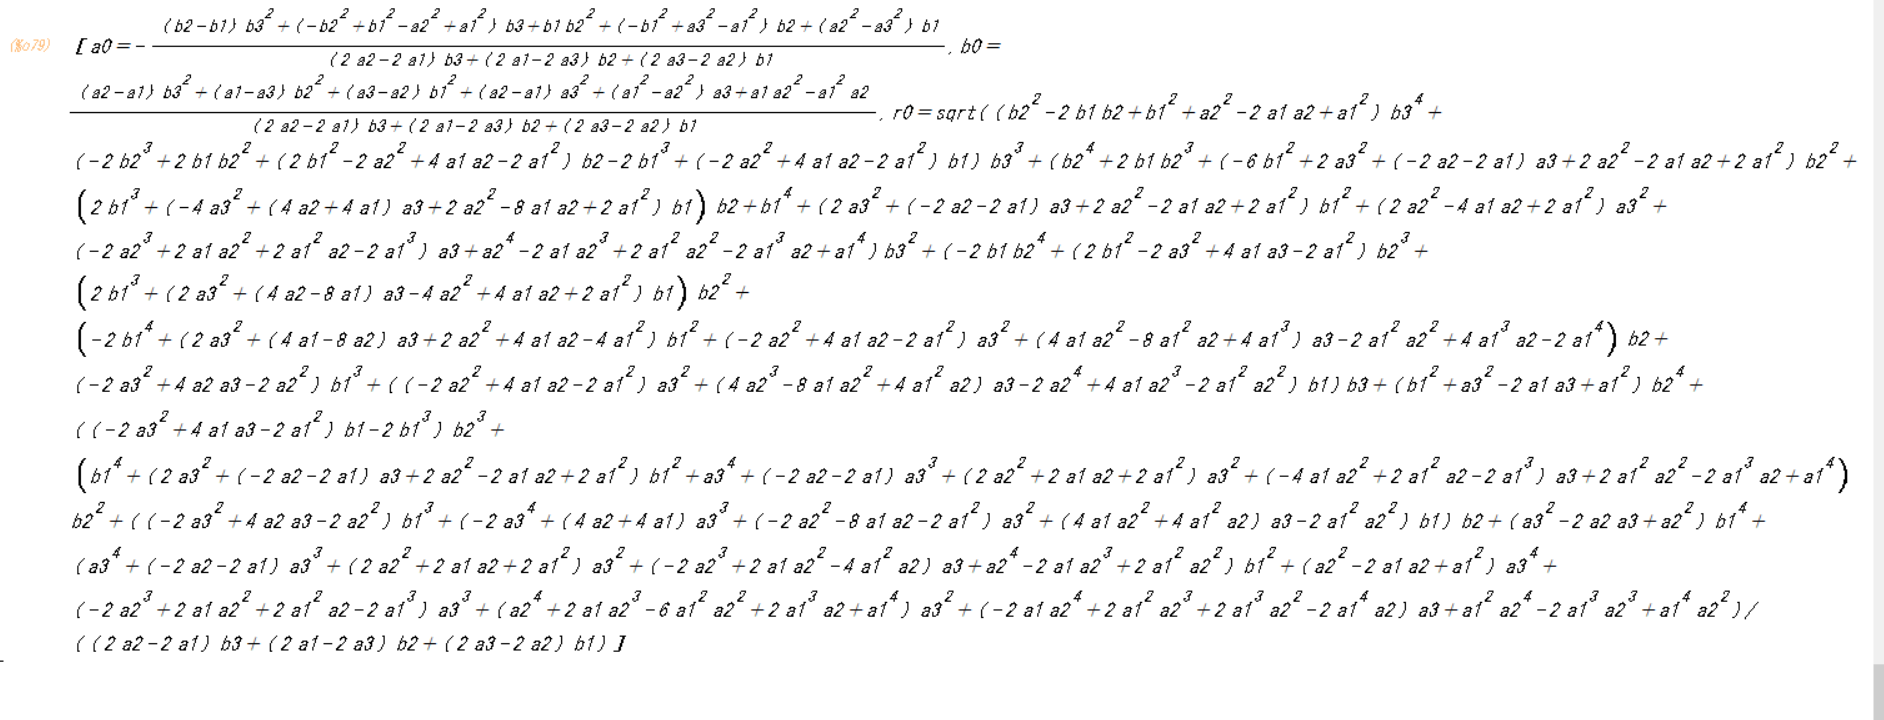
\includegraphics[width=\textwidth]{ReflectionPoincare3Points.png}
 \end{center}
\end{document}